\chapter{Introduction}
\section{Defining disaggregation}
The act of disaggregating something is breaking it into multiple parts. In our case, we are looking to break a signal coming from a single, or multiple sources (see \autoref{chapter-improvements}) into different signals coming from different appliances. Once a signal from an appliance is isolated from the global signal, we would also like to know what signal it is and label it.

\subsection{Non Intrusive Load Monitoring}
Actually what we mean by energy disaggregation is Non Intrusive Load Monitoring (often abbreviated \acrshort{nilm}). Nonintrusive means that we don't have one sensor per appliance, but rather one sensor per electrical network. The purpose of it is to have a simpler installation, fewer costs and an easier way to update the system.

Load monitoring refers to the electrical load, watching it and try to make suppositions about what it means.

\subsection{Different type of devices}
One thing to keep in mind is that there are a lot of different kind of appliances that use electricity in different kind of ways. Not all appliances need a continuous (meaning the same during all the use-time) \acrshort{ac} input at 120V. Actually, there are many types of transformers \cite{harlow2004electric} that don't work the same way and don't necessarily give the same kind of output on a sensor.

There are also appliances that sometimes need a lot of energy, and sometimes don't, like a fridge, an oven or a washing machine. Those appliances often have an identifiable cycle and some studies already address those. But there are also appliances with less predictable cycles, like a drilling machine or other tools.

Waiting for cycles to run in order to identify them could take many minutes, or even hours. This could be a potential problem for some of the applications (see \autoref{section-application})

Having devices using the network in different ways could mean that it would be easy to disaggregate the network, but in practice, it makes it harder because we need multiple ways to collect data, to process them, and eventually make a consensus. This would also mean that the consensus would need to wait for the slowest algorithm to give an output, which would again be a problem for some applications.

Moreover, there are devices that are only in an on/off state and then there are appliances that have multiple states, like a television or a monitor, whose can be on/sleep/off. A laptop or smartphone charger can also have multiple states: on/off but also connected to the laptop or not, and whether the laptop's battery is at full capacity or not.

\section{State of the art}
\subsection{Ways to collect data}
The data collected is most of the time the instantaneous power consumption, but it may also be only the current waveform, or the current waveform combined with instantaneous voltage. Depending on the data we gather, different types of meters and different ways to connect them to the network exist. It may be in parallel or in series, or it may be hard wired to the network or just a clip working with magnetic fields for instance.

A lot of the previous work was focused on slowly acquired data, with the current intensity or more generally the consumed power measured with a sampling rate around 1Hz (like \acrshort{redd}\cite{kolter2011redd}). Others have used a much higher precision to sample the data and even got to a rate of a few GHz \cite{gupta2010electrisense}. This last way to collect data is obviously also much more expensive in hardware: it needs costly measurement tools but it is also harder computationally, needing a faster processor.

Beyond collecting data about the consumption, in order to learn automatically one must also collect data about the state of the appliances. There are various ways to do that. The most used is probably using intrusive sensors, more precisely one sensor per appliance just sensing if that appliance is drawing current from the network or not. In order to eliminate noise, there should be one sensor for every appliance that can send a signal to the nonintrusive sensor.
Some other methods were also designed using thermal imaging \cite{ho2011heatprobe}. This is a bit less intrusive but is also less precise.

There are also multiple public databases if you want to develop an algorithm that needs a lot of data without having to generate it.%http://blog.oliverparson.co.uk/2012/06/public-data-sets-for-nialm.html, http://wiki.nilm.eu/datasets.html




\subsection{Ways to learn}\label{setion:learn}
Like most of the time when building algorithms in artificial intelligence, there are many ways to build a model that will predict the output. All of them have their disadvantages due to the inductive bias and hopefully, most of them have advantages.
\subsubsection{Factorial Hidden Markov Model}
A \acrlong{fhmm} (\acrshort{fhmm}) is a generalization of the \acrshort{hmm} that allows having one \acrshort{hmm} per appliance. \cite{parson2014unsupervised} Each appliance can then have multiple hidden states. This solution has been implemented and tested by J. Zico Kolter and Matthew J. Johnson \cite{kolter2011redd} and gave 64.5\% accuracy on the \acrshort{redd} dataset (around 20 monitored appliances).

The accuracy was computed as the total energy correctly assigned :
\begin{equation}Acc=1-\frac{\sum_{t=1}^{T}\sum_{i=1}^{N}|\hat{y}_t^{(i)}-y_t^{(i)}|}{2\sum_{t=1}^{T} \bar{y}_t}\end{equation}\myequations{Accuracy of total energy correctly assigned}
where $y_t^{(i)}$ is the energy of the $i$th device at time step $t$, $\hat{y}_t^{(i)}$ denotes the algorithm’s prediction for the $i$th device at the $t$th time step, $\bar{y}_t=\sum_{i=1}^{N}y_y^{(i)}$ is the aggregate energy at time step $t$, $N$ the number of appliances, and $T$ is the total number of time steps.

However, an \acrshort{fhmm} needs an exponential number of hidden states: $K^N$ where $K$ is the number of states per appliance and $N$ is the number of appliances. This can become very limiting in real use cases. Some relaxations of the problem exist, like Gibbs sampling, variational Bayes, and variational message passing \cite{parson2014unsupervised}, but this way of solving is still computationally intensive.

\subsubsection{Deep Neural Network}
Deep neural networks are used in a lot of different kinds of applications of machine learning. Some have tried applying this technique to \acrshort{nilm}, with satisfying accuracy on some appliances. The authors of \cite{kelly2015neural} decided to use real data from UK-DALE and generated data in a ratio 50:50 for their experiments. Because neural networks can be trained to detect one appliance, they could test the algorithm on only 5 appliances. In order to keep track of the history of what happens in the network, they used a Recurrent Neural Networks and used small batches of offline disaggregation in order to simulate online disaggregation. They also used a neural network (a \acrlong{dea}, \acrshort{dea}) to remove the noise from the read signal. The results are mitigated; some appliances perform really well on the F1 score but some really don't.

Neural Networks are very expensive to build and need several hours of training per appliance on a current high-end GPU.



\subsubsection{Logical rules}
Sabina Tomkins, Jay Pujara, and Lise Getoor have tried what they call a collective probabilistic approach \cite{tomkins2017disambiguating}. The principle is to group appliances by sets, as some appliances are mostly used together. It should also make it easier to detect as the change on the network is more significant as a set than as a single appliance. Then for each reading and current state, the algorithm outputs a new state. In order to do that, the authors used a \acrlong{hlmrf} (\acrshort{hlmrf})\cite{bach2015hinge}. This algorithm needs a set of soft logical rules, which are in this case based on the duration of use of the appliances, the different sets of appliances used together, the time and date on which the data is read, and others.

The authors have run their algorithm on the \acrshort{redd} and the DATAPORT datasets, and claim to have reduced errors by previous state-of-the-art algorithms by 50\% and 25\% respectively.

One problem with this algorithm is that it computes what we already know. We need to know when an appliance is likely to be used to detect that it is being used. We need to know which sets of appliances are likely being used together in order to detect one of them. It will probably fail to detect that a light is on during the day, that a heater is on during summer or that air conditioning is on in winter. Although, those are pieces of information that can be very useful when we try to disaggregate a signal, depending on the target (see \autoref{section-target})


\subsubsection{Low frequency intensity sampling}\label{section:low-freq}
A patent has already been released on a way to disaggregate electricity using low current sampling by Smappee \cite{bruneel2018energy}. They separated the detection of events and the labelling in two separated tasks. In order to detect events, they measure the power value at regular intervals, $P_t$, and compute the Student's t-test over two larger intervals.
\begin{equation} T(\Delta t_i, \Delta t_j) = \frac{\bar{P_{\Delta t_i}}-\bar{P_{\Delta t_j}}}{\sqrt{\frac{\sigma^2_{\Delta t_i} - \sigma^2_{\Delta t_j}}{n}}} \end{equation}\myequations{T-test for event detection}
Where $\sigma^2_{\Delta t_i}$ is the variance of the power over the time interval $\Delta t_i$. If the t-test has a value above a threshold, an event is detected.
On \autoref{fig:smappe} you can see a schema of an event being detected at time E. In order to know which appliance changed state, they use data from before the event was detected, and data from after. In this data, they locate the lowest and the highest peaks and compute the difference in the power at those two points, $\Delta P_{peak}$, and the time between the two, $\Delta t_{peak}$. They also compute the mean of the \acrshort{dft} (see \autoref{section:ft}) on short intervals before the peak (red area on the picture) and the mean of the the \acrshort{dft} on short intervals after the peak (blue area). With the difference between those two \acrshort{dft} and the information computed about the peaks, they make a decision on which appliance switched its state between ON and OFF.
{\color{red}add similarity function}

The frequency they use for the sampling of the intensity of the current is below 10kHz, which is way below the sampling frequency used in \autoref{section:high-freq} but also way higher than the frequency of time steps used in previous methods. Also, the patent never speaks of any other state for an appliance than ON or OFF.
\begin{figure}
    \centering
    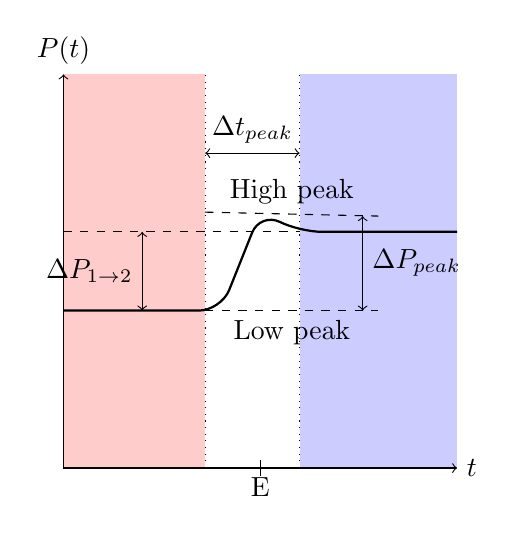
\begin{tikzpicture}
    \fill [red!20!white] (0,0) rectangle (1.8,5);
    \fill [blue!20!white] (3,0) rectangle (5,5);
    \draw[->] (0,0) -- (0,5) node[above] {$P(t)$};
    \draw[->] (0,0) -- (5,0) node[right] {$t$};
    \draw[thick,rounded corners=8pt] (0,2) -- (2,2) -- (2.5,3.25) -- (3,3) -- (5,3);
    \draw[dotted] (1.8,0) -- (1.8,5);
    \draw[dotted] (3,0) -- (3,5);
    \draw[dashed] (1.8,2) -- node[below]{Low peak} (4,2);
    \draw[dashed] (1.8,3.25) -- node[above]{High peak} (4,3.2);
    \draw[dashed] (0,3) -- (3,3);
    \draw[<->] (1.8,4) -- node[above]{$\Delta t_{peak}$} (3,4);
    \draw[<->] (3.8,2) -- node[right] {$\Delta P_{peak}$}(3.8,3.2);
    \draw[<->] (1,2) -- node[left] {$\Delta P_{1\rightarrow2}$}(1,3);
    \draw (2.5,-0.1) -- node[below] {E} (2.5,0.1);
    
    
    \end{tikzpicture}
    \caption{Methodology of Smappee}
    \label{fig:smappe}
\end{figure}


\subsection{Other ways to learn}
Most of the algorithms above only use the power consumption to disaggregate the signal. However we could get a more fine grained data set not only by augmenting the frequency of data acquisition but also by measuring the voltage and the intensity separately.


\subsubsection{Reactive VS Active Power}
Some research \cite{hassan2014empirical} have used the difference between active and reactive power consumption. The reactive power is expressed in Volt-Ampere-Reactive (vars) and is $Q=V_{RMS}I_{RMS}\sin(\phi)$ where $\phi$ is the phase difference between the current and the voltage. The active power is the real power consumed by the appliance. By plotting these powers for multiple appliances we can already see some patterns. Although, an application of this on \acrshort{redd} shows that low active power devices have almost no reactive power and make it difficult to distinguish.

\subsubsection{V-I Trajectory}\label{section-vi}
\begin{wrapfigure}{r}{0.5\textwidth}
    \centering
    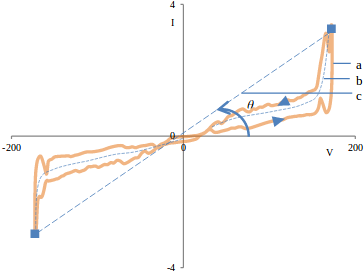
\includegraphics[width=\linewidth]{img/vi-trajectory.png}
    \caption[Graphical illustration of wave-shape metrics]{Graphical illustration of wave-shape metrics:(a) V-I trajectory  (b) Mean curve    (c)  Reference line  joining points  of highest  and lowest  I-coordinate in the V-I plane. \cite{hassan2014empirical}}
    \label{fig:vi-trajectory}
    \vspace{-30pt}
\end{wrapfigure}
\autoref{fig:vi-trajectory} represents the shape of a Voltage-Intensity wave. It is made by measuring the voltage and the intensity multiple times during a cycle of the voltage. \cite{hassan2014empirical} They can be very different according to the working mode of the device. A resistive device would have a V-I trajectory close to the mean curve represented on the figure. A motor would mostly only have a phase difference between volts and amperes so the curve would be an ellipsis. The curve represented on the picture is probably the one of an appliance using a electronic transformer.

This approach can lead to a better separation of the appliances than with a function of reactive and active powers since the later is only a function the first, reducing its dimension.

The features extracted from the shape are as follow \cite{lam2007novel}:
\begin{description}[align=left]
\item[Asymmetry] If an appliance doesn't require as much current in negative and positive cycles, the shape will be asymmetric around the origin of the graph. One way to compute the asymmetry is to use Haudsdroff distance.
\item[Looping direction] The phase angle between the intensity and the voltage determine the looping direction. That phase angle is influenced by capacitors and inductors : capacitors tends to make the curve go clockwise and inductors counter-clockwise. If the appliance is purely resistive, the phase angle will be 0 and there will be no looping direction.
\item[Area] The area is proportionnal to the phase shift, already looked in the looping direction, but still gives more information about an appliance.
\item[Slope of mean line] The mean line is the line joining the points where the voltage is maximum and minimum. It basically gives an estimate of the power consumption.
\item[Self-intersection] When an appliance uses higher harmonic current, there might be multiple intersections in the curve. There is one intersection on \autoref{fig:vi-trajectory} but there would be none on a purely resistive and capacitive appliance for instance, or more, like for a microwave oven. 
\item[Slope of middle segment] The middle segment is the part of the curve where it is \textit{almost} horizontal. When there is a bending point, it becomes the right or the middle segment and the curve becomes more vertical. If there is no bending point, it means that the appliance is probably not a electronic appliance. The slope of the curve in that middle segment can give information on the appliance.
\item[Area of left and right segments] The area depends on the difference of the phase angle of the voltage and the current and the time the current stays at its peak.
\item[Peak of middle segment] The line with the highest difference between the mean line and the curve in its middle segment relative to the current axis is labelled as the peak of the middle segment. The length of that line helps to separate appliances with small power consumption.
\item[Span] It is the difference between the highest and lowest values for the intensity. It helps to estimate the real power of an appliance.
\end{description}

The last item, span, helps determining when an appliance changes state. When a change is detected, the difference between all the items is fed through a classifier (T. Hassan et al. have tried \acrshort{annlm}, \acrshort{annea}, \acrshort{svm} and \acrshort{adaboost}\cite{hassan2014empirical}) to know what appliance it was. 

\subsubsection{k-Nearest Neighbors}\label{section:high-freq}
Once we get to a high enough sampling rate, we can start to get information about the \acrfull{emi} and compare them using the spectrum of this \acrshort{emi}. This is what Sidhant Gupta did with his project, ElectriSense \cite{gupta2010electrisense}. In order to acquire the data, he built a piece of hardware he called FireFly. It is basically a micro computer that monitors one single appliance in an intrusive way. He also monitored the electrical network where he would put the \acrshort{nilm} meter. In order to be synchronised with the different FireFly nodes, all of them are synchronised with the GPS clock.
In order to read the data, he plugs his meter in any electrical socket of the home instead of having to put it on the home electric meter for instance. The meter is composed of a \acrfull{pli} and a \acrfull{usrp}. The \acrshort{pli} is needed in order to filter out the low frequencies, in particular the first harmonics of 60Hz (or other values depending on countries), the frequency of the voltage source. Those frequencies are ignored because they are way too noisy compared to higher frequencies. The \acrshort{usrp} is a device that can sample the analog signal with a sampling frequency up to 1MHz. By using 2048 points in order to compute the \acrshort{fft}, he gets a resolution of 244Hz per FFT bin.

Once the system is set up, the training begins. When an appliance changes its state, the \acrshort{emi} it produces will change on the electrical network, and thanks to the data acquired with the FireFly nodes, the algorithm can label the changes on the network correctly. The data labelled is actually a set of parameters for Gaussian curves fitting the difference between the \acrshort{fft} vector of the \acrshort{emi} before and the \acrshort{fft} vector of the \acrshort{emi} after the appliance changed state.

The training phase produces a lot of training points. Once the training is finished, the FireFly nodes are removed and the labelling process uses a \acrshort{knn} using the parameters of the Gaussian curves as input feature.

Results with this approach depend on the position of the appliances in the home. It will correctly classify two similar lights that are not in the same room but will fail to differentiate them if they are close to another. This is great for the precision of the classification and for many applications but it also means that a learning needs to be done for every single home where we want to run the algorithm.



\cite{do2016applications}%TODO

\section{Applications}\label{section-application}
The purposes of disaggregating such kind of signal are various.

\subsection{Consumption}
The most common purpose is having an estimate of the consumption of each appliance in a household. This means that we don't need to know exactly and immediately when the state of an appliance changes. All we need is that the mean detected uptime of an appliance is close to its true mean uptime. This could help reduce consumption by knowing what appliance is critical. This could also give hints on what appliance could be replaced by a less power consuming one and in how much time the cost can be absorbed by the gain in electricity consumed.

Even if an algorithm is made to be precise in consumption, there are various application requiring different algorithms. If one would need to know at the end of the month what appliance is responsible for the biggest part of the bill is a totally different approach than if one would need to know when and what to unplug because the batteries of a home using only renewable energy are getting low.

\subsection{Security}
Knowing when an appliance with some risks is plugged and on can also be interesting. Using an iron or a hair straightener for too long could mean that someone forgot to plug it off. Detecting this could be interesting. Also, having an air conditioner running in the winter or a heater running in the summer could be a security issue and need to be reported.

\subsection{Home automation}
Other applications could be used in home automation, to turn on or off something when activity is detected on an appliance for instance.


\section{Target}\label{section-target}
If there are multiple applications, there are also multiple targets. One application can have multiple targets and one target can have multiple applications. A target could be a household, an electricity provider or a factory for instance. A household would have a lot of small appliances, with a few energy-consuming devices, and most of the appliances probably use \acrshort{smps} (see \autoref{section-smps}). A factory or a workshop probably uses a lot of high energy-consuming tools and machines.

Such differences are to be taken into account when designing an algorithm.


\section{Application and target VS. Accuracy}
While it may be interesting to have an accuracy as perfect as it may be, one shouldn't forget that the algorithm is made to be used, and instead of trying to improve the accuracy again and again we could improve the usability with regards to various applications of the algorithms. \cite{barker2014nilm} 

If an application only requires to have states that are ON or OFF for the appliances, it may not be fair to compare it with an algorithm that can also detect other states, like transient states for a warm-up or different cycles in a washing machine. An other application might even be further away in terms of evaluation of the accuracy : the estimated consumption of each individual appliance; in that case, we are comparing continuous values and we do not really care of the current state of an appliance.

Also, the type of appliances used in different applications may change the accuracy of an algorithm a lot. If we want to disaggregate the energy consumed in a workshop with a lot of machines using electric motors, or if we want to disaggregate the energy consumed in a home with a lot of appliances using \acrshort{smps} (see \autoref{section-smps}), the accuracy may also be very different. Actually a motor has virtually an infinite number of states varying from rest to full power, but an appliance using \acrshort{smps} generally do not vary much.

If the application requires to be able to disaggregate both devices with high-power and low-power consumption, we will need a different algorithm than one with only similar devices in terms of consumption.

An other import aspect is the time at which we need the data. An algorithm may need to have access to future information to determine if a machine was indeed in a cycle for instance. This is not possible if we try to disaggregate in real time but it is if we collect data for a long time and try to disaggregate it afterwards.

Of course, like for all machine learning algorithms, having one that has a very good accuracy but has a very bad time complexity is not usable in practice. Some algorithms in \autoref{setion:learn} are in exponential complexity, which is usable for a small number of appliances with a modern computer dedicated to it but quickly becomes a problem, and is not computable on a small single boar computer. This use of a computer may be counter productive if the application is to reduce the consumption.


\section{Societal impact}
Today a lot of companies make a lot of their benefits by selling data about our personal life. Even though they shouldn't give access to information that would help identify us, those companies have been known to give away that information to intelligence services when they needed it. While this may seem like a good think in some cases, it still is an infringement of our right to privacy.

The advantages of building a working solution for disaggregation have already been discussed but one shouldn't forget that the data it produces is about our personal life. This means that big companies working with -- and making money from -- this type of data will be very interested in developing this kind of technology. For instance Google has already tried to make its own solution. \cite{googleabandon} 

While this can make a big improvement, amongst other domains, in home automation and energy savings, you could see this as if you gave a camera in your homes to those companies : it can tell whether or not you are at home at a given time and because most of occupations today require electricity it can tell what you are doing. Even though a lot of people have already a camera and a microphone in their home with the stream going straight to those companies like the Kinect from Microsoft or smart televisions, a lot of people are against this type of data being collected.

With this said, not all solutions discussed in this thesis need a central server in order to work, so the collection of data for those big companies would not be direct. However, even solutions that do not need a high computational power use a central server that could collect all the data about the users. \cite{bruneel2018energy}

Now I think that this technology would be really useful but lets not forget about our right to privacy by letting those companies putting one more foot into our lives.



\iffalse
Deep neural networks applied to energy disaggregation\cite{kelly2015neural}

REDD: A public data set for energy disaggregation research\cite{kolter2011redd}

NILM redux: The case for emphasizing applications over accuracy\cite{barker2014nilm}

Nonintrusive load monitoring (NILM) performance evaluation\cite{makonin2015nonintrusive}

An in-depth study into using EMI signatures for appliance identification\cite{gulati2014depth}

ElectriSense: single-point sensing using EMI for electrical event detection and classification in the home\cite{gupta2010electrisense}

HeatProbe: a thermal-based power meter for accounting disaggregated electricity usage\cite{ho2011heatprobe}

Applications of Deep Learning Techniques on NILM\cite{do2016applications}

Approaches to Non-Intrusive Load Monitoring (NILM) in the Home\cite{makonin2012approaches}

Non-intrusive load monitoring approaches for disaggregated energy sensing: A survey\cite{zoha2012non}

Disaggregation of
Domestic Smart Meter Energy Data\cite{kelly2016disaggregation}

Algorithms for Energy Disaggregation\cite{fiol2016algorithms}

A survey on metric learning for feature vectors and structured data\cite{bellet2013survey}

\fi